%Chapter 1
\chapter{Introduction and background}  %J.H Marais, C.J.R. Kriel
\pagenumbering{arabic}
\thispagestyle{empty}
\vspace{38em}
\hrulefill
\\
\enquote{\textit{Precisely one of the most gratifying results of intellectual evolution is the continuous opening up of new and greater prospects.}} -  Nikola Tesla\\
\newpage

\section{Preamble}
This chapter firstly discusses background regarding deep level mining in South Africa. Next, the need to reduce costs of operation in the mining sector is examined. From this, a focus on reducing the energy consumption of compressed air systems is developed. Next, background on compressed air operation and energy interventions are discussed. Simulations and their value in the industry are discussed; leading to a problem statement and objectives of the study. Finally, an overview for the dissertation is provided.
\section{Background on deep level mining}
	\subsection{Mining profitability}
	
	 	Various technical, economic, social and operational challenges are posing a risk to the profitability of the South African mining sector. One of the challenges the sector faces is a rise in the cost of operation \cite{neingo2016trends}.
	 	\par
	 	\footnotetext[1]{Eskom, \enquote{Revenue application - multi year price determination 2013/14 to 2017/18 (mypd3),} [Online] \url{http://www.eskom.co.za/CustomerCare/MYPD3/Documents/NersaReasonsforDecision.pdf, 2013}, [Accessed 22 March 2017].}
	 	
		A considerable factor that is contributing to the increase in operational costs in South African gold mines has been the rise of electricity costs. As shown in \Cref{fig: Eskom tariffs}, the general cost of electricity has increased at a rate greater than inflation since 2008\footnotemark[1].
		
		\footnotetext[2]{inflation.eu, "Historic inflation South Africa." [Online] \url{http://www.inflation.eu/inflation-rates/south-africa/historic-inflation/cpi-inflation-south-africa.aspx}, [Accessed 25 March 2017].}
		\begin{figure}[h]
			\centering
			\fbox{% GNUPLOT: LaTeX picture with Postscript
\begingroup
  \makeatletter
  \providecommand\color[2][]{%
    \GenericError{(gnuplot) \space\space\space\@spaces}{%
      Package color not loaded in conjunction with
      terminal option `colourtext'%
    }{See the gnuplot documentation for explanation.%
    }{Either use 'blacktext' in gnuplot or load the package
      color.sty in LaTeX.}%
    \renewcommand\color[2][]{}%
  }%
  \providecommand\includegraphics[2][]{%
    \GenericError{(gnuplot) \space\space\space\@spaces}{%
      Package graphicx or graphics not loaded%
    }{See the gnuplot documentation for explanation.%
    }{The gnuplot epslatex terminal needs graphicx.sty or graphics.sty.}%
    \renewcommand\includegraphics[2][]{}%
  }%
  \providecommand\rotatebox[2]{#2}%
  \@ifundefined{ifGPcolor}{%
    \newif\ifGPcolor
    \GPcolortrue
  }{}%
  \@ifundefined{ifGPblacktext}{%
    \newif\ifGPblacktext
    \GPblacktextfalse
  }{}%
  % define a \g@addto@macro without @ in the name:
  \let\gplgaddtomacro\g@addto@macro
  % define empty templates for all commands taking text:
  \gdef\gplbacktext{}%
  \gdef\gplfronttext{}%
  \makeatother
  \ifGPblacktext
    % no textcolor at all
    \def\colorrgb#1{}%
    \def\colorgray#1{}%
  \else
    % gray or color?
    \ifGPcolor
      \def\colorrgb#1{\color[rgb]{#1}}%
      \def\colorgray#1{\color[gray]{#1}}%
      \expandafter\def\csname LTw\endcsname{\color{white}}%
      \expandafter\def\csname LTb\endcsname{\color{black}}%
      \expandafter\def\csname LTa\endcsname{\color{black}}%
      \expandafter\def\csname LT0\endcsname{\color[rgb]{1,0,0}}%
      \expandafter\def\csname LT1\endcsname{\color[rgb]{0,1,0}}%
      \expandafter\def\csname LT2\endcsname{\color[rgb]{0,0,1}}%
      \expandafter\def\csname LT3\endcsname{\color[rgb]{1,0,1}}%
      \expandafter\def\csname LT4\endcsname{\color[rgb]{0,1,1}}%
      \expandafter\def\csname LT5\endcsname{\color[rgb]{1,1,0}}%
      \expandafter\def\csname LT6\endcsname{\color[rgb]{0,0,0}}%
      \expandafter\def\csname LT7\endcsname{\color[rgb]{1,0.3,0}}%
      \expandafter\def\csname LT8\endcsname{\color[rgb]{0.5,0.5,0.5}}%
    \else
      % gray
      \def\colorrgb#1{\color{black}}%
      \def\colorgray#1{\color[gray]{#1}}%
      \expandafter\def\csname LTw\endcsname{\color{white}}%
      \expandafter\def\csname LTb\endcsname{\color{black}}%
      \expandafter\def\csname LTa\endcsname{\color{black}}%
      \expandafter\def\csname LT0\endcsname{\color{black}}%
      \expandafter\def\csname LT1\endcsname{\color{black}}%
      \expandafter\def\csname LT2\endcsname{\color{black}}%
      \expandafter\def\csname LT3\endcsname{\color{black}}%
      \expandafter\def\csname LT4\endcsname{\color{black}}%
      \expandafter\def\csname LT5\endcsname{\color{black}}%
      \expandafter\def\csname LT6\endcsname{\color{black}}%
      \expandafter\def\csname LT7\endcsname{\color{black}}%
      \expandafter\def\csname LT8\endcsname{\color{black}}%
    \fi
  \fi
    \setlength{\unitlength}{0.0500bp}%
    \ifx\gptboxheight\undefined%
      \newlength{\gptboxheight}%
      \newlength{\gptboxwidth}%
      \newsavebox{\gptboxtext}%
    \fi%
    \setlength{\fboxrule}{0.5pt}%
    \setlength{\fboxsep}{1pt}%
\begin{picture}(9360.00,4032.00)%
    \gplgaddtomacro\gplbacktext{%
      \colorrgb{0.00,0.00,0.00}%
      \put(682,1144){\makebox(0,0)[r]{\strut{}$0$}}%
      \colorrgb{0.00,0.00,0.00}%
      \put(682,1422){\makebox(0,0)[r]{\strut{}$5$}}%
      \colorrgb{0.00,0.00,0.00}%
      \put(682,1701){\makebox(0,0)[r]{\strut{}$10$}}%
      \colorrgb{0.00,0.00,0.00}%
      \put(682,1979){\makebox(0,0)[r]{\strut{}$15$}}%
      \colorrgb{0.00,0.00,0.00}%
      \put(682,2258){\makebox(0,0)[r]{\strut{}$20$}}%
      \colorrgb{0.00,0.00,0.00}%
      \put(682,2536){\makebox(0,0)[r]{\strut{}$25$}}%
      \colorrgb{0.00,0.00,0.00}%
      \put(682,2814){\makebox(0,0)[r]{\strut{}$30$}}%
      \colorrgb{0.00,0.00,0.00}%
      \put(682,3093){\makebox(0,0)[r]{\strut{}$35$}}%
      \colorrgb{0.00,0.00,0.00}%
      \put(682,3371){\makebox(0,0)[r]{\strut{}$40$}}%
      \colorrgb{0.00,0.00,0.00}%
      \put(814,924){\makebox(0,0){\strut{}$2006$}}%
      \colorrgb{0.00,0.00,0.00}%
      \put(2172,924){\makebox(0,0){\strut{}$2008$}}%
      \colorrgb{0.00,0.00,0.00}%
      \put(3530,924){\makebox(0,0){\strut{}$2010$}}%
      \colorrgb{0.00,0.00,0.00}%
      \put(4888,924){\makebox(0,0){\strut{}$2012$}}%
      \colorrgb{0.00,0.00,0.00}%
      \put(6246,924){\makebox(0,0){\strut{}$2014$}}%
      \colorrgb{0.00,0.00,0.00}%
      \put(7604,924){\makebox(0,0){\strut{}$2016$}}%
      \colorrgb{0.00,0.00,0.00}%
      \put(8962,924){\makebox(0,0){\strut{}$2018$}}%
    }%
    \gplgaddtomacro\gplfronttext{%
      \csname LTb\endcsname%
      \put(176,2257){\rotatebox{-270}{\makebox(0,0){\strut{}\% increase}}}%
      \put(4888,594){\makebox(0,0){\strut{}Year}}%
      \put(4888,3701){\makebox(0,0){\strut{}Electricity price increases in South Africa}}%
      \csname LTb\endcsname%
      \put(6770,393){\makebox(0,0)[r]{\strut{}Eskom general tariff increases (\%)}}%
      \csname LTb\endcsname%
      \put(1493,1562){\makebox(0,0){\strut{}6.0}}%
      \put(2172,2759){\makebox(0,0){\strut{}27.5}}%
      \put(2851,2970){\makebox(0,0){\strut{}31.3}}%
      \put(3530,2608){\makebox(0,0){\strut{}24.8}}%
      \put(4209,2664){\makebox(0,0){\strut{}25.8}}%
      \put(4888,2118){\makebox(0,0){\strut{}16.0}}%
      \put(5567,1673){\makebox(0,0){\strut{}8.0}}%
      \put(6246,1673){\makebox(0,0){\strut{}8.0}}%
      \put(6925,1673){\makebox(0,0){\strut{}8.0}}%
      \put(7604,1673){\makebox(0,0){\strut{}8.0}}%
      \put(8283,1673){\makebox(0,0){\strut{}8.0}}%
      \csname LTb\endcsname%
      \put(6770,173){\makebox(0,0)[r]{\strut{}Inflation rate in south Africa (\%)}}%
    }%
    \gplbacktext
    \put(0,0){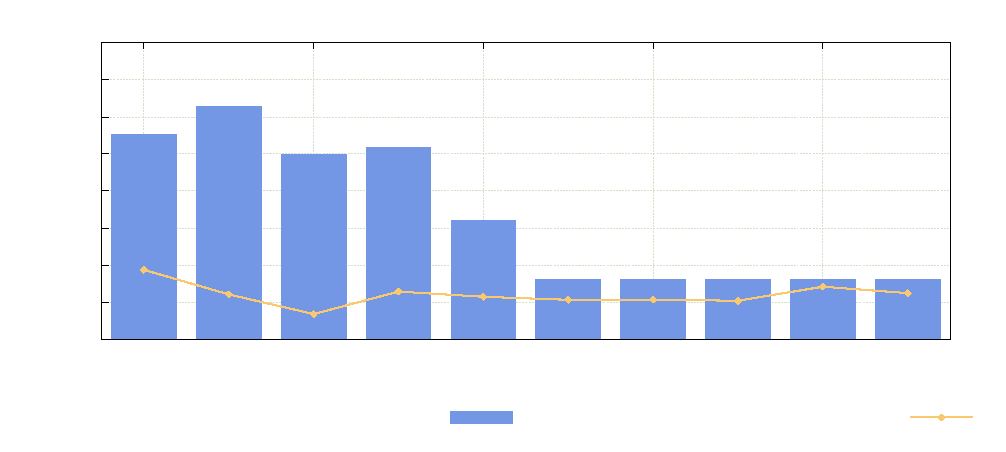
\includegraphics{Graphs/1/Eskom/Eskom}}%
    \gplfronttext
  \end{picture}%
\endgroup
}
			\caption[Electricity price increases between 2007 and 2017 compared to the inflation rate in South Africa]{Electricity price increases between 2007 and 2017\protect\footnotemark[1] compared to the inflation rate in South Africa\protect\footnotemark[2]}
			\label{fig: Eskom tariffs}
		\end{figure}
	%%%%%%%%%%%%%%%%%%%%%%%%%%%%%%%%%%%%%%
	\clearpage
	%%%%%%%%%%%%%%%%%%%%%%%%%%%%%%%%%%%%%%
		\par
		In addition to rising electricity costs, gold ore grades of South African mines have fallen substantially over the last few decades \cite{mudd2007global}. As ore grades decline, the energy utilised per unit of metal increases exponentially \cite{muller2010numerical}. 
		\par
		Additionally, mines are having to extend their operations deeper in order to reach the valuable ore reefs [CITATION NEEDED]. Therefore, mines require significantly more energy per unit of metal produced. This combination of tariff increases and increased energy usage per unit have led to significant rises in mining operation costs.
	\subsection{Process of a deep level mine}
	South Africa's mines are some of the deepest in the world. Some mine shafts are reaching depths greater than $4000m$ below the surface \cite{vosloo2012case}. The process of extracting ore at this depth is dependent on the essential services, mainly cooling and ventilation, pumping, compressed air and hoisting, as shown in \Cref{fig: Mining Layout}.
	\par 
	 Cooling and ventilation systems are required to maintain a safe working temperature underground. Pumping is critical to remove service and fissure water, preventing flooding. Compressed air is used to power underground drills and machines safely. A hoisting system is needed to bring the ore to the surface and to transport workers in the mine. The hoisted materials are transferred to a plant for processing.  
		\begin{figure}[h!]
			\centering
			\fbox{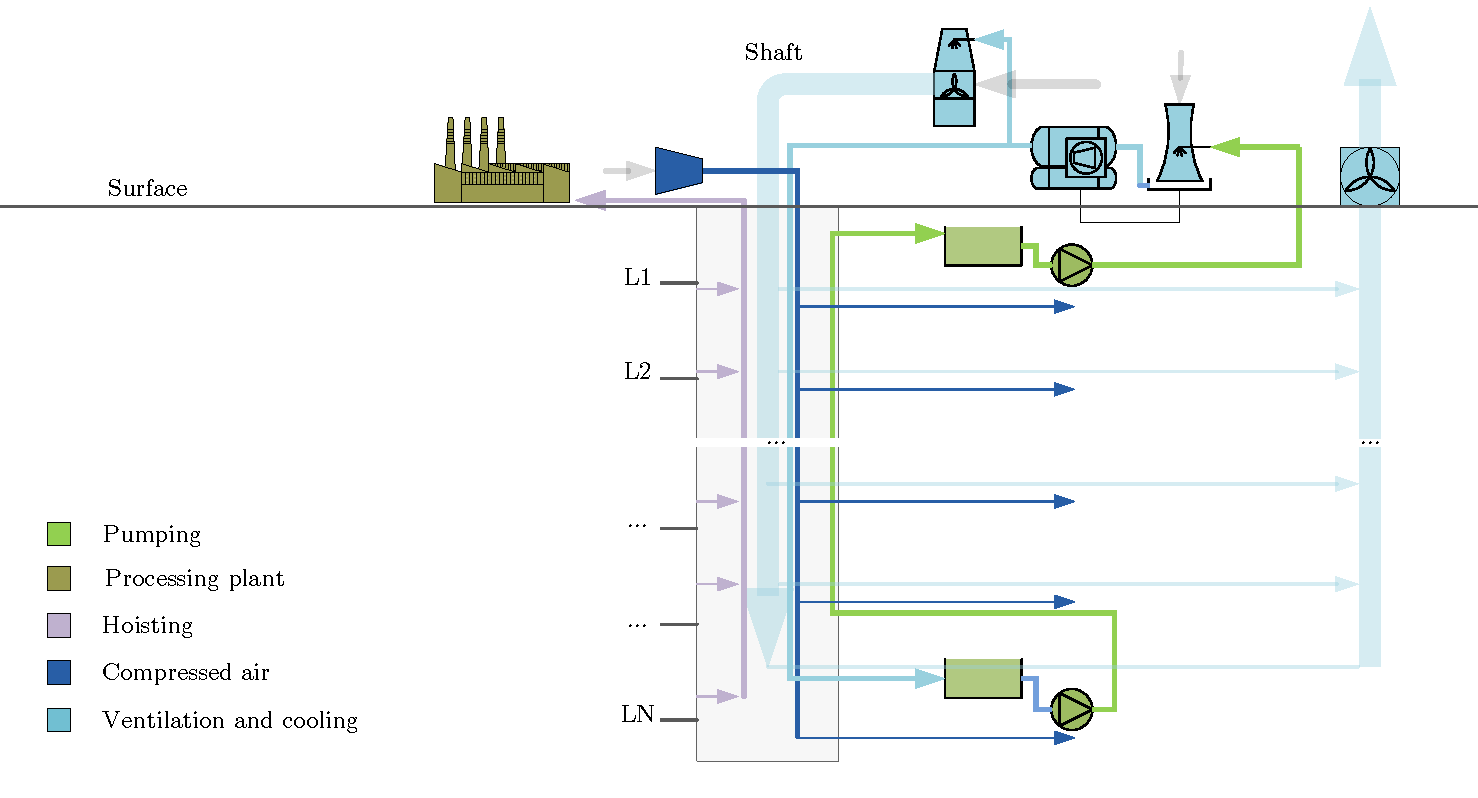
\includegraphics[width=\textwidth]{Graphs/1/Layout/Layout.pdf}}
			\caption{A schematic showing the mining processes.}
			\label{fig: Mining Layout}
		\end{figure}
		\subsection{Energy usage of mining services}
		\footnotetext[1]{Eskom, \enquote{The energy efficiency series - towards an energy efficient mining sector,} [Online] \url{http://www.eskom.co.za/sites/idm/Documents/121040ESKD}, February 2010, [Accessed 19 March 2017].}
		
			The mining industry uses X MW of Energy [Citation needed]. In South Africa, the industry utilises approximately 15\% of the national electricity supplier's annual output, of which, gold and platinum mines use 80\%\footnotemark[1].
			\par
			 \Cref{fig: Energy Split} illustrates the division of energy use within the mining industry. The chart indicates that compressed air systems utilise the most energy within a mine. Therefore, energy can be most effectively reduced through the implementation of energy saving interventions on compressed air systems.
			 %%%%%%%%%%% Explain other parameters on graph
			\begin{figure}[h]
				\centering
				\fbox{% GNUPLOT: LaTeX picture with Postscript
\begingroup
  \makeatletter
  \providecommand\color[2][]{%
    \GenericError{(gnuplot) \space\space\space\@spaces}{%
      Package color not loaded in conjunction with
      terminal option `colourtext'%
    }{See the gnuplot documentation for explanation.%
    }{Either use 'blacktext' in gnuplot or load the package
      color.sty in LaTeX.}%
    \renewcommand\color[2][]{}%
  }%
  \providecommand\includegraphics[2][]{%
    \GenericError{(gnuplot) \space\space\space\@spaces}{%
      Package graphicx or graphics not loaded%
    }{See the gnuplot documentation for explanation.%
    }{The gnuplot epslatex terminal needs graphicx.sty or graphics.sty.}%
    \renewcommand\includegraphics[2][]{}%
  }%
  \providecommand\rotatebox[2]{#2}%
  \@ifundefined{ifGPcolor}{%
    \newif\ifGPcolor
    \GPcolortrue
  }{}%
  \@ifundefined{ifGPblacktext}{%
    \newif\ifGPblacktext
    \GPblacktextfalse
  }{}%
  % define a \g@addto@macro without @ in the name:
  \let\gplgaddtomacro\g@addto@macro
  % define empty templates for all commands taking text:
  \gdef\gplbacktext{}%
  \gdef\gplfronttext{}%
  \makeatother
  \ifGPblacktext
    % no textcolor at all
    \def\colorrgb#1{}%
    \def\colorgray#1{}%
  \else
    % gray or color?
    \ifGPcolor
      \def\colorrgb#1{\color[rgb]{#1}}%
      \def\colorgray#1{\color[gray]{#1}}%
      \expandafter\def\csname LTw\endcsname{\color{white}}%
      \expandafter\def\csname LTb\endcsname{\color{black}}%
      \expandafter\def\csname LTa\endcsname{\color{black}}%
      \expandafter\def\csname LT0\endcsname{\color[rgb]{1,0,0}}%
      \expandafter\def\csname LT1\endcsname{\color[rgb]{0,1,0}}%
      \expandafter\def\csname LT2\endcsname{\color[rgb]{0,0,1}}%
      \expandafter\def\csname LT3\endcsname{\color[rgb]{1,0,1}}%
      \expandafter\def\csname LT4\endcsname{\color[rgb]{0,1,1}}%
      \expandafter\def\csname LT5\endcsname{\color[rgb]{1,1,0}}%
      \expandafter\def\csname LT6\endcsname{\color[rgb]{0,0,0}}%
      \expandafter\def\csname LT7\endcsname{\color[rgb]{1,0.3,0}}%
      \expandafter\def\csname LT8\endcsname{\color[rgb]{0.5,0.5,0.5}}%
    \else
      % gray
      \def\colorrgb#1{\color{black}}%
      \def\colorgray#1{\color[gray]{#1}}%
      \expandafter\def\csname LTw\endcsname{\color{white}}%
      \expandafter\def\csname LTb\endcsname{\color{black}}%
      \expandafter\def\csname LTa\endcsname{\color{black}}%
      \expandafter\def\csname LT0\endcsname{\color{black}}%
      \expandafter\def\csname LT1\endcsname{\color{black}}%
      \expandafter\def\csname LT2\endcsname{\color{black}}%
      \expandafter\def\csname LT3\endcsname{\color{black}}%
      \expandafter\def\csname LT4\endcsname{\color{black}}%
      \expandafter\def\csname LT5\endcsname{\color{black}}%
      \expandafter\def\csname LT6\endcsname{\color{black}}%
      \expandafter\def\csname LT7\endcsname{\color{black}}%
      \expandafter\def\csname LT8\endcsname{\color{black}}%
    \fi
  \fi
    \setlength{\unitlength}{0.0500bp}%
    \ifx\gptboxheight\undefined%
      \newlength{\gptboxheight}%
      \newlength{\gptboxwidth}%
      \newsavebox{\gptboxtext}%
    \fi%
    \setlength{\fboxrule}{0.5pt}%
    \setlength{\fboxsep}{1pt}%
\begin{picture}(9360.00,3528.00)%
    \gplgaddtomacro\gplbacktext{%
      \colorrgb{0.00,0.00,0.00}%
      \put(682,440){\makebox(0,0)[r]{\strut{}$0$}}%
      \colorrgb{0.00,0.00,0.00}%
      \put(682,1005){\makebox(0,0)[r]{\strut{}$5$}}%
      \colorrgb{0.00,0.00,0.00}%
      \put(682,1569){\makebox(0,0)[r]{\strut{}$10$}}%
      \colorrgb{0.00,0.00,0.00}%
      \put(682,2134){\makebox(0,0)[r]{\strut{}$15$}}%
      \colorrgb{0.00,0.00,0.00}%
      \put(682,2698){\makebox(0,0)[r]{\strut{}$20$}}%
      \colorrgb{0.00,0.00,0.00}%
      \put(682,3263){\makebox(0,0)[r]{\strut{}$25$}}%
      \colorrgb{0.00,0.00,0.00}%
      \put(1323,150){\makebox(0,0){\strut{}\scriptsize{\shortstack{Compressed \\ air}}}}%
      \colorrgb{0.00,0.00,0.00}%
      \put(2342,150){\makebox(0,0){\strut{}\scriptsize{\shortstack{Mining \\ processes}}}}%
      \colorrgb{0.00,0.00,0.00}%
      \put(3360,150){\makebox(0,0){\strut{}\scriptsize{\shortstack{Pumping}}}}%
      \colorrgb{0.00,0.00,0.00}%
      \put(4379,150){\makebox(0,0){\strut{}\scriptsize{\shortstack{Ventilation \\ and cooling}}}}%
      \colorrgb{0.00,0.00,0.00}%
      \put(5397,150){\makebox(0,0){\strut{}\scriptsize{\shortstack{Buildings \\ and hostels}}}}%
      \colorrgb{0.00,0.00,0.00}%
      \put(6416,150){\makebox(0,0){\strut{}\scriptsize{\shortstack{Processing \\ plant}}}}%
      \colorrgb{0.00,0.00,0.00}%
      \put(7434,150){\makebox(0,0){\strut{}\scriptsize{\shortstack{Hoisting}}}}%
      \colorrgb{0.00,0.00,0.00}%
      \put(8453,150){\makebox(0,0){\strut{}\scriptsize{\shortstack{Other}}}}%
    }%
    \gplgaddtomacro\gplfronttext{%
      \csname LTb\endcsname%
      \put(176,1851){\rotatebox{-270}{\makebox(0,0){\strut{}\% of total energy consumption}}}%
    }%
    \gplbacktext
    \put(0,0){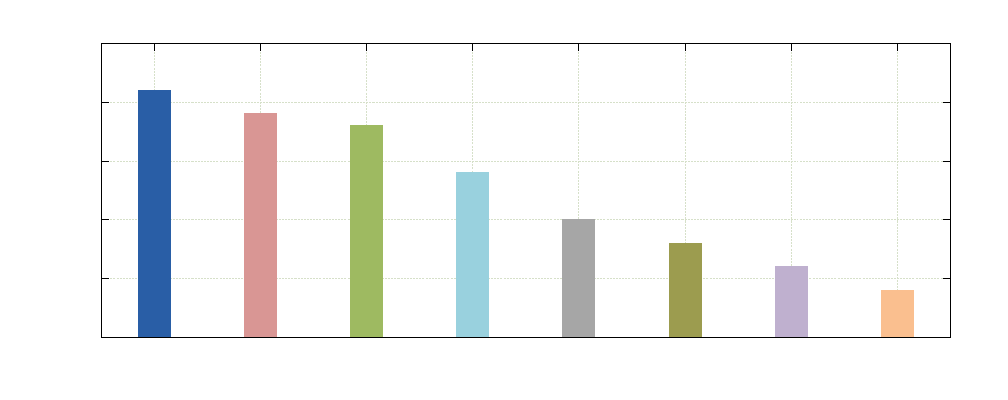
\includegraphics{Graphs/1/distribution/distribution}}%
    \gplfronttext
  \end{picture}%
\endgroup
}
				\caption[The percentagee energy consumption for each mining system]{The percentage energy consumption for each mining system \cite{le2005energy}}
				\label{fig: Energy Split}
			\end{figure}
\section{Compressed air systems in mining}
	\subsection{Compressed air in operation}\label{key}
		Largely due to their reliability, versatilely and ease of use, the South African mining industry has installed extensive compressed air networks. These systems can have compressors with capacities of up to 15 Megawatt ($MW$)\cite{Marais2012PhD}. However, the supply of compressed air is a high energy demanding and costly process \cite{padachi2009energy}.
		\par 
		The energy used for compressed air production contributes to between 9\% and 20\% of the total mining energy consumption\footnotemark[1] \cite{du2011development}. Additionally, the compression process is highly inefficient. It has been estimated that the efficiency of the process of converting electrical energy to power pneumatic drills is as low as 4\% \cite{fraser2008saving}.
		\par
		Large compressed air systems are likely inefficient. Internationally, the expected energy savings potential of a large compressed air network has been proven to be 15\% \cite{neale2009compressed}. Marais \cite{marais2013simplification} showed that energy efficiency interventions could lead to energy and cost savings of between 30\% and 40\%. 
		
	\subsection{Inefficiencies found in compressed air systems}
		Compressed air distribution networks in the mining industry consist of multiple compressors and working areas up to eight kilometres away from the source on the surface \cite{Marais2012PhD}. Due to their size and complexity, these systems are prone to significant energy losses [Citation Needed].
		\par 
		Compressed air leakage accounts for as much as 35\% of the energy losses of a compressed air network \cite{Lawrence2004Improving}. Other systemic losses include, faulty valves, pipe diameter fluctuations, obstructed air compressor intake filters and inefficient compressors. 	
		\par
		Leakage and inefficiency detection strategies are not often pursued in the South African mining industry \cite{vanTonder2010Masters}. Many mines do however perform leak inspections either internally or by an outside company. In these inspections, an ultrasonic detector is used to locate the leak. 
		\par 
		Alternatively, some mines employ the \enquote{walk and listen} method to identify leaks from the audible sound that it produces \cite{vanTonder2010Masters}. Once the inspection is completed, the findings, including the locations and estimated costs of all identified leaks, are reported.
		
	\subsection{Compressed air savings interventions}
		From literature, it has been observed that energy saving interventions on compressed air systems have historically implemented one or a combination of following strategies \cite{Snyman2011Masters}:
		\begin{itemize}
			\item Reduce leaks
			\item Reduce demand
			\item Reduce unauthorised air usage
			\item Increase supply efficiency
			\item Optimise supply
		\end{itemize}
	 Often a combination of energy strategies will lead to the most savings \cite{Marais2012PhD}. In \Cref{Chap2}, successfully completed compressed air interventions on mining systems will be discussed from literature.
	 \par 
	 Once an energy saving measure has been identified, it is most often necessary to make estimations to determine the potential costs and benefits of the intervention. The estimations have typically been performed using first principle calculations, simplified mathematical models and practical tests where possible. 
	 \par 
	 However, new tools have enabled quick, accurate compressed air model development. Through simulations, accurate estimations can be obtained quickly, with no risk and at comparatively low resource requirement.
\section{Use of simulation in industry }
	\subsection{Background on industrial simulation}
	
		Continuous improvements in computing hardware have led to major advancement in software technology. Consequently, the use of computational simulation has become an increasingly valuable tool for many industries \cite{kocsis2003integration}.
		\par 
		In \textit{ Handbook of Simulation: Principles, methodology, advances, applications, and practice}, the advantages of the use of simulation in the industry are discussed as follows \cite{banks1998handbook}: %%% Chapter 1 of book
		\begin{itemize}
			\item The ability to test new policies, operating procedures and methods without disrupting the actual system.
			\item The means to identify problems in complex systems by gathering insight in the interactions within the system.
			\item The facility to compress or expand time to investigate phenomena thoroughly.
			\item The capability to determine the limits and constraints within a system.
			\item The potential to build consensus about proposed designs or modifications.
		\end{itemize}

	\subsection{Simulation usage in compressed air optimisation}
		Simulation has been used to test and identify energy and operational improvement modifications in mining compressed air systems. However, in the past producing complex models for mining systems was not feasible as simulation software required difficult to obtain data inputs \cite{marais2013simplification}. 
		\par 
		\subsubsection{Simplified "vessel" model}
		Before new software tools allowed for the development of detailed mining compressed air simulation models, Marais \cite{Marais2012PhD}, \cite{marais2013simplification} created a simplified compressed air model to estimate and quantify the performance of potential energy interventions. Marais simplified the mining compressed air system, comparing the network to an air source and a vessel with many leaks. The simplified model is illustrated in \Cref{fig:Marais vessel model}.
		\begin{figure}[h!]
			\centering
			\fbox{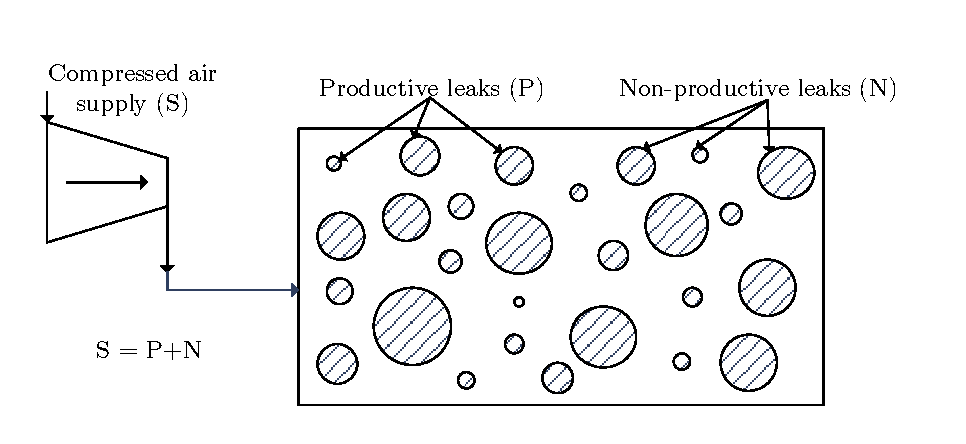
\includegraphics[trim= 0 0.4cm 0 0.8cm, width=\textwidth]{Images/2/marais/Vessel}}
			\caption[Simplified compressed air netowrk model]{Simplified compressed air network model. Adapted from Marais \cite{Marais2012PhD}.}
			\label{fig:Marais vessel model}
		\end{figure}
		\par 
		A calculation methodology was developed to estimate the expected energy savings impact on the system quickly. From this, energy saving estimations and rules were designed as listed in \Cref{table: Rules of thumb}. 
		\par 
		\begin{table}[h]
			\centering
			\begin{tabular}{p{0.4\textwidth}p{0.05\textwidth}p{0.5\textwidth}}
				\hline
				Intervention && Estimation rule\\
				\hhline{===} 
				Reducing compressor deliver pressure & & $x \%$ pressure reduction $\propto$ (1.6 to 1.8)$\cdot x\%$ power reduction \newline \\
				Reduce control valve pressure & &$x \%$ pressure reduction $\propto$ $p\cdot x\%$ power reduction. \newline \newline Where p is the valves' relative flow contribution to the system \newline \\
				Reduction of flow && $x \%$ flow reduction $\propto x \%$ power reduction \newline\\
				\hline
			\end{tabular} 
			\caption[Summary of energy saving estimation rules]{Summary of energy saving estimation rules \cite{Marais2012PhD}.}
			\label{table: Rules of thumb}
		\end{table}
		There is not a high degree of precision in this approach as specific details regarding the air network are not taken into account. The simplified approach cannot be used to estimate more complex scenarios. The method also does not estimate other potential benefits of interventions such as pressure delivery improvements.
		
		\subsubsection{Simplified air network model}
		Kriel \cite{Kriel2014Masters} used simulation to estimate the performance of energy projects on mine compressed air systems. The KYPipe GAS software tool was utilised to develop simulation models for the systems. Kriel simplified the air networks for the simulations to a single compressor representing the supply processes and an outlet flow to each underground level in the network. The model is shown graphically in \Cref{fig:kriel model}
		\begin{figure}[h!]
			\centering
			\fbox{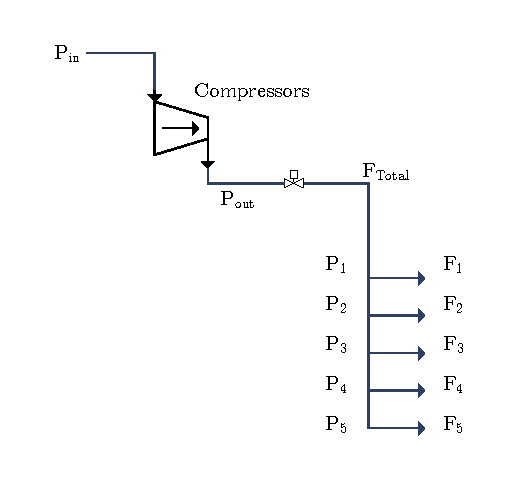
\includegraphics[trim = -2cm 0.5cm -2cm 0.5cm ,width=\textwidth]{Images/2/kriel/model}}
			\caption[Simplified system model]{Simplified system model. Adapted from Kriel \cite{Kriel2014Masters}}
			\label{fig:kriel model}
		\end{figure}
		\par 
		The simulation was performed to quantify the savings from underground network interventions. The interventions were designed to reduce flow to the network. The estimated savings from the simulations varied between 10 and 25\% compared to the actual performance of the interventions. Like the vessel model discussed previously, the simplified air network model can not be used to estimate the energy savings potential of more complex scenarios.
		\par 
		 The simulation procedure in this study could be improved by using a more detailed model and a more precise verification method. The method could lead to savings predictions with higher accuracy. 
		\par
		The use of planned manual measurements, estimations and new software technologies can be used to develop more detailed compressed air models \cite{Bredenkamp2015Challeges}, \cite{Mare2017Evaluating}. Using a structured procedure may allow for the development of more detailed and accurate mine compressed air simulations.
		
		%A standard procedure for developing and verifying simulation has also not been developed.

\section{Problem statement and objectives}
	\subsection{Problem statement}
 		Rising costs and falling ore grades are driving the mining industry to reduce operational costs. The industry can save significant energy cost through interventions in compressed air systems. However, manual testing of these interventions is risky and cumbersome.
 		\par
 		Computer modelling and simulation of compressed air systems can be used to quantify and prioritise operational interventions with minimal risk. However, integrated simulations have not been used to their full potential in compressed air system studies in the past. With new tools and more detailed simulation models, the energy and operational efficiency of mining compressed air systems can be improved, leading to significant energy and cost savings as well as other potential improvements for a mine's operation.
 		\par 
 		Therefore, a need exists for an integrated compressed air simulation approach to identify energy and operational improvements for mines.
 			\subsection{Research objectives}
 			
 			%%%%%% Not Good
		The main aim of this dissertation is to identify energy savings through the identification of operational improvements in mining compressed air systems. A simulation process will be developed to achieve this goal.The other objectives for this study are:
		\begin{itemize}
			\item Develop an integrated approach to develop an implement compressed air simulations;
			\item Use simulations to apply and rank compressed air operation interventions;
			\item Model mining compressed air networks components accurately
			\item Develop an approach to verify compressed air simulation models
		\end{itemize}
		
\section{Dissertation overview}
	\paragraph{Chapter 1} \hspace{0.4cm} - \hspace{0.05cm} This chapter serves as an introduction to the dissertation. The chapter provides the relevant background in mining, compressed air and simulation to establish the problem statement. The objectives of the study are then outlined.
	\paragraph{Chapter 2} \hspace{0.4cm} - \hspace{0.05cm} Chapter 2 provides a review of the literature and necessary background relevant to the study. The chapter firstly provides background on mining compressed air networks. A review of compressed air energy interventions is then performed. A review of simulation usage in the mining industry then follows. Finally, a review of simulation usage in mining compressed air systems.
	\paragraph{Chapter 3} \hspace{0.4cm} - \hspace{0.05cm} Chapter 3 provides a simulation methodology. The method outlines the processes used to investigate a compressed air system, develop and calibrate simulation models and finally to implement simulations and obtain results.
	\paragraph{Chapter 4} \hspace{0.4cm} - \hspace{0.05cm} Chapter 4 provides validation of the methodology through case study results. Results of three case studies are provided. Finally, the impact of large scale implementation of the simulation methodology is discussed.
	\paragraph{Chapter 5} \hspace{0.4cm} - \hspace{0.05cm} Chapter 5 concludes the dissertation. The chapter also provides recommendations for further studies regarding compressed air simulation.
	%\texttt{Describe (in approximately one sentence each) the contents of \\each of the dissertation chapters. No results here.}
